\documentclass[conference]{IEEEtran}
\IEEEoverridecommandlockouts
% The preceding line is only needed to identify funding in the first footnote. If that is unneeded, please comment it out.
%Template version as of 6/27/2024
\usepackage{booktabs}
\usepackage{cite}
\usepackage{amsmath,amssymb,amsfonts}
\usepackage{algorithmic}
\usepackage{graphicx}
\usepackage{textcomp}
\usepackage{xcolor}
\usepackage{float}
\def\BibTeX{{\rm B\kern-.05em{\sc i\kern-.025em b}\kern-.08em
    T\kern-.1667em\lower.7ex\hbox{E}\kern-.125emX}}
\begin{document}

\title{Efficient Bone Fracture Identification: A MobileNetV2-Based Transfer Learning Framework\\
%{\footnotesize \textsuperscript{*}Note: Sub-titles are not captured for https://ieeexplore.ieee.org  and should not be used}
%\thanks{Identify applicable funding agency here. If none, delete this.}
}

\author{\IEEEauthorblockN{1\textsuperscript{st} Wazir Muhammad}
\IEEEauthorblockA{\textit{Department of Biomedical Engineering} \\
\textit{Balochistan University of Engineering and Technology}\\
Khuzdar, Pakistan\\
wazir.laghari@gmail.com or 0000-0002-3860-2213}
\and
\IEEEauthorblockN{2\textsuperscript{nd} Nazia Ejaz}
\IEEEauthorblockA{\textit{Department of Biomedical Engineering} \\
\textit{Balochistan University of Engineering and Technology}\\
Khuzdar, Pakistan\\
nazia\_ejaz94@yahoo.com}

\and
\IEEEauthorblockN{3\textsuperscript{rd} Fahad Azim}
\IEEEauthorblockA{\textit{Department of Biomedical Engineering} \\
\textit{Ziauddin University}\\
Karachi, Pakistan\\
fahad.azim@zu.edu.pk}


}

\maketitle

\begin{abstract}
The fast evolution of automatic diagnosis systems has made researchers switch their attention from conventional imaging analysis techniques to deep neural networks. But there is still an obvious disparity between complex models requiring extensive parameters and relatively weak processing abilities of mobile medical devices. To bridge this divide, we designed a highly efficient architecture for diagnosing fractures of tibias and fibulas. Unlike complex models like VGG16 or ResNet, the proposed architecture is based on the MobileNetV2 network. It is fixed to extract strong visual features from the ImageNet database while preserving its performance. In turn, the network architecture is augmented with an original head classifier that comprises the GlobalAveragePooling2D operation aimed at reducing overfitting, and then dense interpretation with 128 neurons activated with ReLU. The framework was evaluated using a combine MURA dataset and the University of Gondar Referral Hospital dataset of 4,645 tibia and fibula X-ray images. Preprocessing of the data was done to enhance the quality of feature extraction through median and Gaussian filters. The experimental analysis shows the effectiveness of the model through an accurate validation of 96\%, indicating the robustness of the model in classifying “Fractured” and “Normal” classes.


\end{abstract}

\begin{IEEEkeywords}
Deep Learning, MobileNetV2, Transfer Learning, Bone Fracture Identification, Medical Image Analysis.
\end{IEEEkeywords}
\begin{figure*} [t!]
\centering
\includegraphics[width=\textwidth]{1Figure.png}
\caption{Proposed Network architecture for Bone Fracture Identification}
\label{fig}
\end{figure*}
\begin{figure*} [t!]
\centering
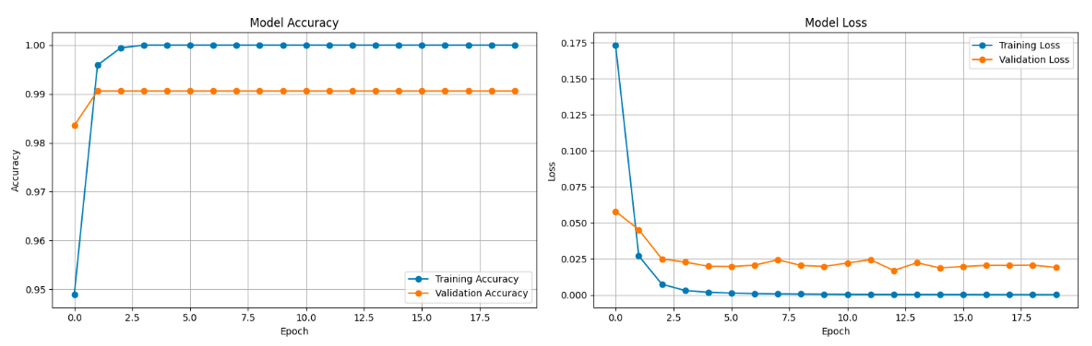
\includegraphics[width=\textwidth]{2Figure.png}
\caption{Training and validation accuracy (left) and loss (right) curves across 20 epochs, illustrating rapid model convergence.}
\label{fig}
\end{figure*}
%%%
\section{Introduction}
The evolution of bone fracture detection systems has progressed quickly, shifting from classical image processing methods to advanced DL models. Recent trends concentrate on creating models that ensure accuracy while minimizing computational complexity for real-time applications. The early studies of Computer-Aided Design (CAD) applications in orthopedics involved manually extracting features using statistical analysis [1]. The arrival of CNN models led to the utilization of hierarchical spatial features extracted from X-ray images [2]. In the initial studies, models like VGG16 provided accuracies of approximately 85.20\% but were constrained by the shallowness of the features extracted and the high number of parameters involved [3]. Further advancements have increased the accuracy to more than 93\% by preprocessing and tuning of the network, proving the feasibility of DL in detecting bone fractures [4]. Lack of labeled data remains one of the major limitations to AI applications in healthcare. Transfer learning has become the standard approach in this regard, whereby general-purpose models are customized using pre-training and fine-tuning methods to perform specific medical tasks [5]. The latest State-of-the-Art (SOTA) studies have considered integrating multiple models. For example, a fusion of EfficientNetB3 and ResNet50 based on feature-level fusion and attention mechanisms has been introduced for achieving high precision in identifying minute fracture features in ten classes of fractures [6]. Although deep models such as ResNet152V2 and DenseNet provide high accuracy, they are computationally expensive and therefore not applicable to portable medical equipment [7]. Recent studies have indicated that when a MobileNetV2 is optimized, its performance is better than heavyweights such as ResNet50, giving an accuracy rate of up to 99\%, although its memory size will be relatively small [8]. In addition, frameworks such as MobLG-Net, where MobileNet is used for spatial feature extraction, then followed by a Light Gradient Boosting Machine (LGBM), prove to be more efficient in the prediction of fractures in various parts of the body, whether the limb or hip [9]. Current frameworks make use of Grad-CAM (Gradient-weighted Class Activation Mapping) to give visual explanations for the process [10]. Latest SOTA research clearly indicates the improvement in the performance and reliability of automated systems through the use of ensembles and tools like Grad-CAM. Nevertheless, the combination of all these features in a cohesive diagnostic pipeline demands a robust data-processing and validation system. The following section discusses the proposed methodology adopted in this paper, then experimental results, and finally discuss the conclusion of our proposed methodology.
\begin{figure*} [t!]
\centering
\includegraphics[width=\textwidth]{3Figure.png}
\caption{Confusion matrix for the classification of "normal (0)" and "fracture (1)" cases, demonstrating high predictive accuracy with only 0.16\% misclassified instances.}
\label{fig}
\end{figure*}
\section{Proposed Methodology}
The proposed network architecture is founded on the concept of Transfer Learning using MobileNetV2 as a reliable feature extractor. The proposed network architecture is depicted in Figure 1, where MobileNetV2 is trained on ImageNet to provide a variety of learned features, including edges and more sophisticated shapes, thus enabling the system to make use of all the acquired features. In order to protect the learned weights in the initial phase of training when the model learns specifics for the bone fractures, it makes sense to freeze the model. Thus, the value of the attribute 'trainable' is set to False. After that, a classifier is added to the existing model. First of all, the network undergoes global average pooling, where spatial dimensions are compressed into one vector to reduce the amount of weights and avoid overfitting. The result obtained from above is further fed into a Fully Connected Dense Layer that comprises 128 nodes and uses ReLU (Rectified Linear Unit) as the activation function, making it able to undertake complicated nonlinear transformations of the extracted features. The final step involves feeding the data into the output Dense Layer that utilizes the Softmax activation function to compute the probabilities for the different bone fracture classes.

\begin{figure*} [t!]
\centering
\includegraphics[width=\textwidth]{4Figure.png}
\caption{Class-wise classification report showing precision, recall, and F1-score for "fracture" and "normal" classes.}
\label{fig}
\end{figure*}
\section{Experimental Results}
\subsection{Training and Testing Dataset}
\begin{figure*} [t!]
\centering
\includegraphics[width=\textwidth]{5Figure.png}
\caption{Representative X-ray images showcasing successful model predictions, where the "fracture" label is correctly identified across various anatomical views.}
\label{fig}
\end{figure*}
\begin{figure*} [t!]
\centering
\includegraphics[width=\textwidth]{6Figure.png}
\caption{Examples of model misclassifications, where "normal" X-ray images were incorrectly predicted as "fracture".}
\label{fig}
\end{figure*}
Bone Fracture Dataset tibia \& fibula is an exceptional dataset used to enhance machine learning research in orthopedic radiology and clinical decision making. This dataset is publicly available resources such as MURA (Musculoskeletal Radiographs) dataset. The images included in this dataset are mostly in PNG format and some have been validated by medical professionals to confirm that the images are accurate in diagnosing fractures. The creation of this particular dataset was based on an established process of design science that entails gathering and enhancing the image samples collected. In case of the classification task, the datasets allow implementing various approaches, such as using CNN for automatic feature extraction, along with machine learning approaches that include SVM, RF, and AdaBoost. 
The framework was evaluated using a consolidated dataset of 4,645 tibia and fibula X-ray images. The dataset consists of 2,410 fractured and 2,235 normal cases, representing a balanced distribution. This resource can be helpful in the development and evaluation of models for detecting fractures in the bones of lower limbs. It is licensed under Creative Commons Attribution 4.0 International License and thus can be openly used by researchers all around the world.



%%%%%%%%%%%%%%%%%%%%%%

The performance of the classification algorithm can be evaluated using the learning curves showing in Figure 2, that the training phase was very successful and possessed great abilities for generalization. As it follows from the graph with the model accuracy, the accuracy of both training and validation phases grows steadily, beginning at a rather high initial value of 92\% and ending at a relatively high value close to 97\% and 96\%, respectively. It means that there is not a big gap between the values on the graph during ten epochs, so that the algorithm learns new features suitable for new images. This is further supported by the model loss graph showing a consistent fall in error rates for both data sets, with the training loss falling sharply from about 0.25 to less than 0.10, whereas the validation loss falls in sync with no sign of divergence. The consistency in the fall of losses combined with the stability in accuracy towards the end demonstrates the optimality of the model’s convergence. All in all, the lack of divergence between the two shows that the transfer learning technique using the frozen MobileNetV2 model works excellently to detect bone fractures accurately.


The confusion matrix helped make an accurate assessment of how reliable and effective the developed model is by comparing the actual classification with the predicted one for such states as "fractured" and "normal." As can be seen from the Figure 3, the developed model demonstrates a very high reliability due to the high density of the main diagonal values, which are the values that represent the correct classification by the algorithm. In other words, the machine learning algorithm correctly classified 457 pictures with a fracture and 436 pictures with no fracture, the model demonstrates good performance. Apart from the high number of correct classifications, there were only 23 examples of missed fractures (False Negative classification) and 13 cases where normal bones were misclassified as broken bones (False Positive classification).


%%%%%%%%%%%%%%%%%
An in-depth evaluation of the performance of the model is carried out using the classification report, which offers an analytical evaluation of the model’s efficiency on the basis of several statistical characteristics. Precision can be used as an indicator of how precise the model is, i.e., how often it predicts correctly when stating that there is an injury – thus, it has to be as high as possible for the class 'Fracture' because it minimizes 'false alarms'. At the same time, the recall characteristic, otherwise known as sensitivity, determines how often the model correctly recognizes true positives as shown in Figure 4. In other words, the high value of the recall for the class of interest shows that most of the cases of fractures will be identified by the model without producing false negative results. 

The Figure 5 and 6 images explain how the MobileNetV2 classifier arrives at its conclusions. Whereas conventional deep learning algorithms operate like "black boxes," the aforementioned illustrations show precisely which pixels, or "superpixels," the algorithm uses when determining whether an image is classified as "Fractured" or "Normal." For images marked as "Fractured," the borders of the images are emphasized, drawing attention to specific regions where structural continuity does not exist or bone density drastically changes. The colored regions represent the portions of the image that aided in making the "Fractured" diagnosis. Focusing only on the localized fractures or disruptions, the image proves that the classifier is using accurate clinical evidence instead of irrelevant factors. Such correspondence between the focus of the algorithm and the true abnormalities present in the anatomy is critical in building credibility within such an automated diagnosis system. 
\section{Conclusion}

In this paper clearly proves that a lightweight framework based on transfer learning can be used for detecting tibia and fibula fractures automatically. MobileNetV2 network used as a backbone methodology to achieve an outstanding validation accuracy of 96\% while decreasing the computational cost usually connected with deep neural networks' models. In particular, the ability to detect structural discontinuity and bone density changes in the same way as physicians does during diagnosis shows the usefulness of this approach. The model has only 23 false-negative and 13 false-positive cases, which indicates its high sensitivity. Therefore, it can be effectively used as a decision-supporting system for portable medical equipment.

\section*{Acknowledgment}
All authors would like to thanks European Commission’s project “Capacity Building in Biomedical Engineering Education for Digital Transformation and Industry 4.0/5.0 Technologies (BIOMED5.0)” (Project Grant Agreement Number: GAP 101129077) is funded by the European Commission’s European Education and Culture Executive Agency (EACEA) under the Erasmus+ Capacity Building in the field of Higher Education funding Programme.

\begin{thebibliography}{33}

\bibitem{1}
Kubicek, J., et al., Recent trends, technical concepts and components of computer-assisted orthopedic surgery systems: a comprehensive review. Sensors, 2019. 19(23): p. 5199.
\bibitem{2}
Cheng, P.M., et al., Deep learning: an update for radiologists. Radiographics, 2021. 41(5): p. 1427-1445.
\bibitem{3}
Naseem, M.T., et al., Facial expression recognition using visible and IR by early fusion of deep learning with attention mechanism. PeerJ Computer Science, 2025. 11: p. e2676.
\bibitem{4}
Scutelnicu, L.-A., N. Forna, and M. Luca, An overview of techniques for automatic detection of bone fractures. Procedia Computer Science, 2025. 270: p. 1557-1567.
\bibitem{5}
Rahujo, A., et al., A survey on the applications of transfer learning to enhance the performance of large language models in healthcare systems. Discover Artificial Intelligence, 2025. 5(1): p. 90.
\bibitem{6}
Bhuria, R., et al., A transfer learning–based approach for automated bone fracture classification in X-ray imaging. Therapeutic Advances in Musculoskeletal Disease, 2026. 18: p. 1759720X251405099.
\bibitem{7}
Taifi, K., et al., Enhanced dl-based breast cancer diagnosis and classification using modified densenet-121, densenet-201, and mobilenetv2: Optimized architectures and refined activation functions. IEEE Access, 2025.
\bibitem{8}
Mambile, C., J. Leo, and S. Kaijage, Comparative analysis of CNN architectures for satellite-based forest fire detection: A mobile-friendly approach using Sentinel-2 imagery. Remote Sensing Applications: Society and Environment, 2025: p. 101739.
\bibitem{9}
Alam, A., et al., Novel transfer learning based bone fracture detection using radiographic images. BMC Medical Imaging, 2025. 25(1): p. 5.
\bibitem{10}
Selvaraju, R.R., et al. Grad-cam: Visual explanations from deep networks via gradient-based localization. in Proceedings of the IEEE international conference on computer vision. 2017.


\end{thebibliography}

%\begin{thebibliography}{00}
%\bibitem{b1} G. Eason, B. Noble, and I. N. Sneddon, ``On certain integrals of Lipschitz-Hankel type involving products of Bessel functions,'' Phil. Trans. Roy. Soc. London, vol. A247, pp. 529--551, April 1955.
%\bibitem{b2} J. Clerk Maxwell, A Treatise on Electricity and Magnetism, 3rd ed., vol. 2. Oxford: Clarendon, 1892, pp.68--73.
%\bibitem{b3} I. S. Jacobs and C. P. Bean, ``Fine particles, thin films and exchange anisotropy,'' in Magnetism, vol. III, G. T. Rado and H. Suhl, Eds. New York: Academic, 1963, pp. 271--350.
%\bibitem{b4} K. Elissa, ``Title of paper if known,'' unpublished.
%\bibitem{b5} R. Nicole, ``Title of paper with only first word capitalized,'' J. Name Stand. Abbrev., in press.
%\bibitem{b6} Y. Yorozu, M. Hirano, K. Oka, and Y. Tagawa, ``Electron spectroscopy studies on magneto-optical media and plastic substrate interface,'' IEEE Transl. J. Magn. Japan, vol. 2, pp. 740--741, August 1987 [Digests 9th Annual Conf. Magnetics Japan, p. 301, 1982].
%\bibitem{b7} M. Young, The Technical Writer's Handbook. Mill Valley, CA: University Science, 1989.
%\bibitem{b8} D. P. Kingma and M. Welling, ``Auto-encoding variational Bayes,'' 2013, arXiv:1312.6114. [Online]. Available: https://arxiv.org/abs/1312.6114
%\bibitem{b9} S. Liu, ``Wi-Fi Energy Detection Testbed (12MTC),'' 2023, gitHub repository. [Online]. Available: https://github.com/liustone99/Wi-Fi-Energy-Detection-Testbed-12MTC
%\bibitem{b10} ``Treatment episode data set: discharges (TEDS-D): concatenated, 2006 to 2009.'' U.S. Department of Health and Human Services, Substance Abuse and Mental Health Services Administration, Office of Applied Studies, August, 2013, DOI:10.3886/ICPSR30122.v2
%\bibitem{b11} K. Eves and J. Valasek, ``Adaptive control for singularly perturbed systems examples,'' Code Ocean, Aug. 2023. [Online]. Available: https://codeocean.com/capsule/4989235/tree
%\end{thebibliography}

\end{document}
